\section{(3.8)}
% A farmer is considering a pipe-pump assembly to irrigate a field during the summer. The 
% water source is an underground well, 250 feet deep, with the highest free water surface 
% approximately 8 feet below grade. To minimize pump operation time, the farmer plans to fill 
% a 2,500-gallon tank within 4 hours, providing adequate water for farm operations. The vented 
% cylindrical tank must be no more than 10 feet in length and should include valved piping 
% connections. The tank can be placed at any suitable location within the system. Given the 
% field and well's location, the pumps must be positioned no more than 600 feet from the well. 
% The pipe will connect to an existing irrigation system, which is 750 feet from the well and 
% has a 10-foot length. The terrain from the well to the field is flat. Please complete the 
% following tasks: 
% (1) Design a constant cross-area piping system that includes 2 pumps. Specify the pipe size, 
% pipe length, pipe material, pump sizes, and necessary piping accessories to meet the farmer’s 
% water requirements. For pump selection, you may refer to Taco pumps: 
% http://www.tacocomfort.com/product-category/pumps/. Performance curves for the pumps 
% can be found in the "Related Documents/Data Sheets" section for each series on the website. 
% Other pump brands are also acceptable. Please attach the selected pump performance curve 
% to your assignment. 
% (2) Specify the maximum depth of the pipe inlet within the well. 
% Further Information: Consider using a foot valve at the inlet to ensure proper pump priming.
\textit{A farmer is considering a pipe-pump assembly to irrigate a field during the summer. The water source is an underground well, 250 feet deep, with the highest free water surface approximately 8 feet below grade. To minimize pump operation time, the farmer plans to fill a 2,500-gallon tank within 4 hours, providing adequate water for farm operations. The vented cylindrical tank must be no more than 10 feet in length and should include valved piping connections. The tank can be placed at any suitable location within the system. Given the field and well's location, the pumps must be positioned no more than 600 feet from the well. The pipe will connect to an existing irrigation system, which is 750 feet from the well and has a 10-foot length. The terrain from the well to the field is flat. Please complete the following tasks:}

\paragraph{(1)} \textit{Design a constant cross-area piping system that includes 2 pumps. Specify the pipe size, pipe length, pipe material, pump sizes, and necessary piping accessories to meet the farmer’s water requirements. For pump selection, you may refer to Taco pumps: http://www.tacocomfort.com/product-category/pumps/. Performance curves for the pumps can be found in the "Related Documents/Data Sheets" section for each series on the website. Other pump brands are also acceptable. Please attach the selected pump performance curve to your assignment.}

\paragraph{(2)} \textit{Specify the maximum depth of the pipe inlet within the well.}

\subsection{Assumptions}
\begin{itemize}
    \item Temp is room temperature, 70$^\circ$F
    \item Irrigation system is same size as connected pipe
    \item Pipe is A40 steel
    \item Use friction loss of < 3 ft/100ft
    \item Constant pipe size
    \item Ball valves used at inlet
    \item All connections are threaded
    \item All bends 90$^\circ$
    \item Foot valve used at inlet
    \item Constant pipe size
    \item Flow velocity is 5 fps, pump station line max, lower than erosion limit
    \item Sharp edge exit \& entry
\end{itemize}

\subsection{Sketch}
\begin{figure}[H]
    \centering
    
\includegraphics[width=0.9\textwidth]{Questions/Figures/Q2 Sketch.png}
\end{figure}

\subsection{Analysis: Pump Selection}
\subsubsection{Pipe Sizing}
The flow rate can be calculated as:
\begin{align*}
    Q & = \frac{2500 \; \text{gallons}}{4 \; \text{hours}} \cdot \frac{1 \; \text{hour}}{60 \; \text{min}}         \\
      & = 10.42 \; \text{gpm}                                                                                      \\
      & = 10.42 \cdot \frac{1 \; \text{ft}^3}{7.48 \; \text{gallons}} \cdot \frac{1 \; \text{min}}{60 \; \text{s}} \\
      & = 0.0232 \; \text{ft}^3/\text{s}
\end{align*}
From pipe diameter can be determined since the pipe length is sketched to be 10ft:
\begin{align*}
    V_{\text{cylinder}} & = \frac{\pi D^2}{4} \cdot L                                                                                                     \\
    \implies D          & = \sqrt{\frac{4 V_{\text{cylinder}}}{\pi L}}                                                                                    \\
                        & = \sqrt{\frac{4 \cdot 2500 \; \text{gallons}}{\pi \cdot 10 \; \text{ft}}} \cdot \frac{1 \; \text{ft}^3}{7.48 \; \text{gallons}} \\
                        & = 2.53 \; \text{ft}
\end{align*}
On chart in Figure A.4, a pipe of 1.5 inch diameter will result in a water velocity of 1.8 fps, friction loss of 1.5 ft/100ft. A threaded connection is applicable for this use.

\subsubsection{Reynolds Number}
The Reynolds number for the pipe can be calculated as:
\begin{align*}
    \text{Re} & = \frac{\rho v D}{\mu} = \frac{62.3 \times 1.8 \times 1.5/12}{6.556 \times 10^{-4}} \\
              & = 2.1 \times 10^5
\end{align*}
This flow is turbulent.

\subsubsection{Energy Balance}
For pump 1:
\begin{align*}
    h_{1-p_1} = \frac{1.5}{100} \left(160 + 220 + 200\right) = 8.7 \; \text{ft}
\end{align*}
and pump 2:
\begin{align*}
    h_{1-p_2} = \frac{1.5}{100} \left(170 + 150 + 10\right) = 4.95 \; \text{ft}
\end{align*}
Minor losses:
\begin{align*}
    k_{\text{foot valve}}     & = 1.25  \\
    k_\text{exit}             & = 1     \\
    k_\text{entrance}         & = 0.5   \\
    k_{\text{elbow 90}^\circ} & = 1.225 \\
    k_{\text{ball valve}}     & = 0.05
\end{align*}
for pump 1:
\begin{align*}
    h_{lm} & = \frac{v^2}{2g} \sum k_L                                                                                                    \\
           & =  \frac{v^2}{2g} \left(k_{\text{foot valve}} + 2 k_{\text{elbow 90}^\circ} + 3 k_{\text{ball valve}} + k_\text{exit}\right) \\
           & = \frac{1.8^2}{2 \cdot 32.2} \left(1.25 + 2 \cdot 1.225 + 3 \cdot 0.05 + 1\right)                                            \\
           & = 0.244 \; \text{ft}
\end{align*}
and for pump 2:
\begin{align*}
    h_{lm} & = \frac{v^2}{2g} \sum k_L                                                                                                   \\
           & =  \frac{v^2}{2g} \left(k_{\text{entracnce}} + 2 k_{\text{elbow 90}^\circ} + 3 k_{\text{ball valve}} + k_\text{exit}\right) \\
           & = \frac{1.8^2}{2 \cdot 32.2} \left(0.5 + 2 \cdot 1.225 + 3 \cdot 0.05 + 1\right)                                            \\
           & = 0.206 \; \text{ft}
\end{align*}

total head loss:
\begin{align*}
    h_{lt, p_1} & = 8.7 + 0.244 = 8.94 \; \text{ft}  \\
    h_{lt, p_2} & = 4.95 + 0.206 = 5.16 \; \text{ft}
\end{align*}

Assume $P_1$ is full tank. $P_2 = P_{\text{atm} + \rho g d} = P_{\text{atm} + \rho g (z_2 - z_1 - x)}$. Also set $v_1 = v_2$ since constant diameter pipe. Letting $z_1$ be 0,
\begin{align*}
    h_{p_1} & = \left(\frac{P_\text{atm} + \rho g D}{\rho g} + \alpha \frac{v^2}{2g} + z_2 \right) - \left(\frac{P_\text{atm} + \rho g (z_2 - z_1 - 8)}{\rho g} + \alpha \frac{v^2}{2g} + z_1\right) + h_{lt, p_1} \\
            & = D + x + h_{lt, p_1}
\end{align*}
Let $x = 8$ ft, and $x = 160$ ft in worse case
\begin{align*}
    h_{p_1} & = 6.53 + 8 + 8.94 = 23.47 \; \text{ft}   \\
    h_{p_1} & = 6.53 + 160 + 8.94 = 171.7 \; \text{ft}
\end{align*}

For pump 2, assume $P_3 = P_\text{atm} = P_4$, $v_3 = v_4$. $z_3 = z_4$. Then,
\begin{align*}
    h_{p_2} & = \left(\frac{P_\text{atm} + \rho g D}{\rho g} + \alpha \frac{v^2}{2g} + z_2 \right) - \left(\frac{P_\text{atm}}{\rho g} + \alpha \frac{v^2}{2g} + z_1\right) + h_{lt, p_2} \\
    h_{p_2} & = h_{lt, p_2} = 5.16 \; \text{ft}
\end{align*}

\subsubsection{Pump Requirements}
For pump 1:
\begin{itemize}
    \item $\sim 11$ gpm
    \item 140 FT
    \item large pump head
    \item mounted is mosts suitable
\end{itemize}
\begin{figure}[H]
    \centering
    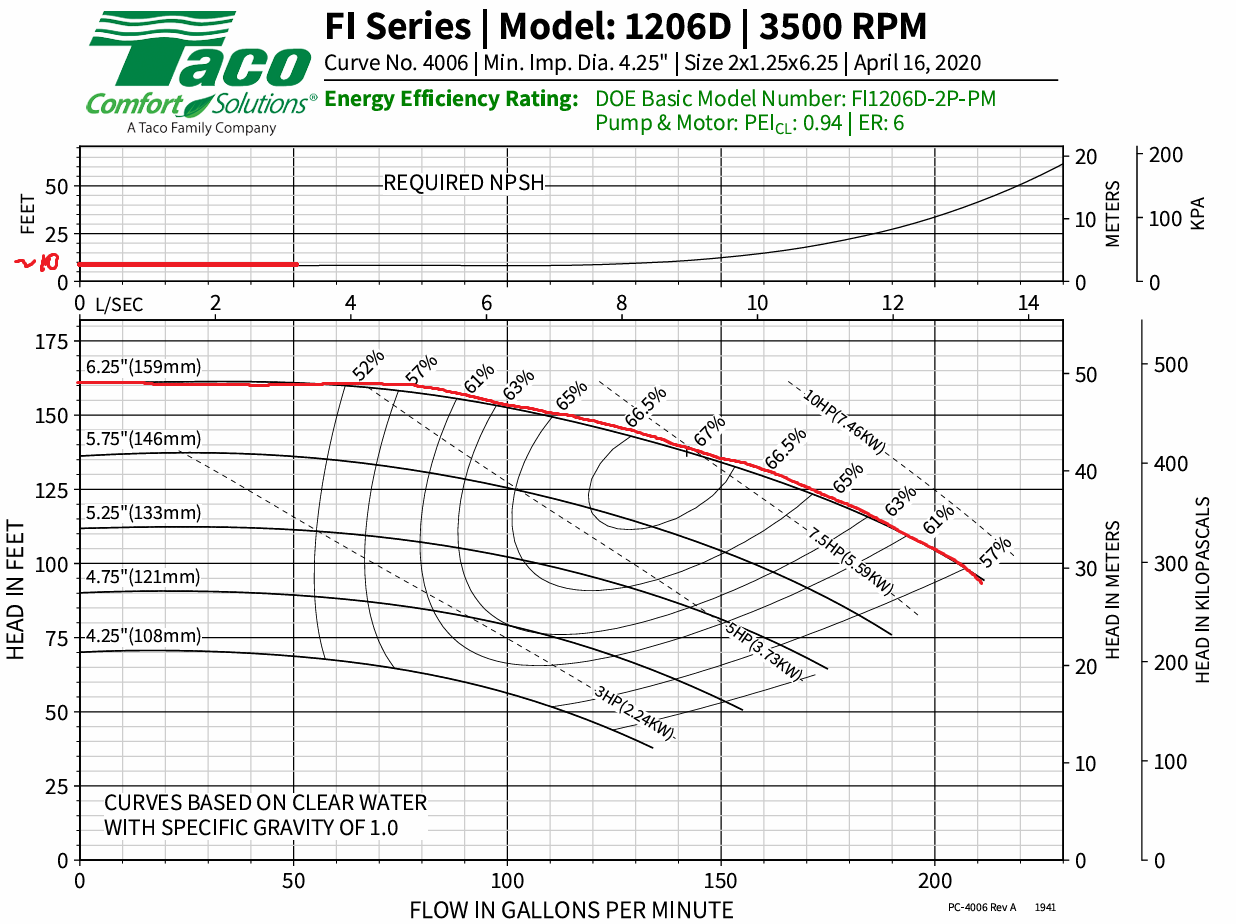
\includegraphics[width=0.9\textwidth]{Questions/Figures/Q2 Pump 1.png}
\end{figure}
This pump is suitable for the application,
\begin{itemize}
    \item Casing size: 2'' x 1.25 '' x 7.25''
    \item Impeller D: 6.25''
    \item Motor: 10 hp (oversized)
    \item Motor speed: 3500 rpm
    \item NPSHR: 10 ft
\end{itemize}

For pump 2:
\begin{figure}[H]
    \centering
    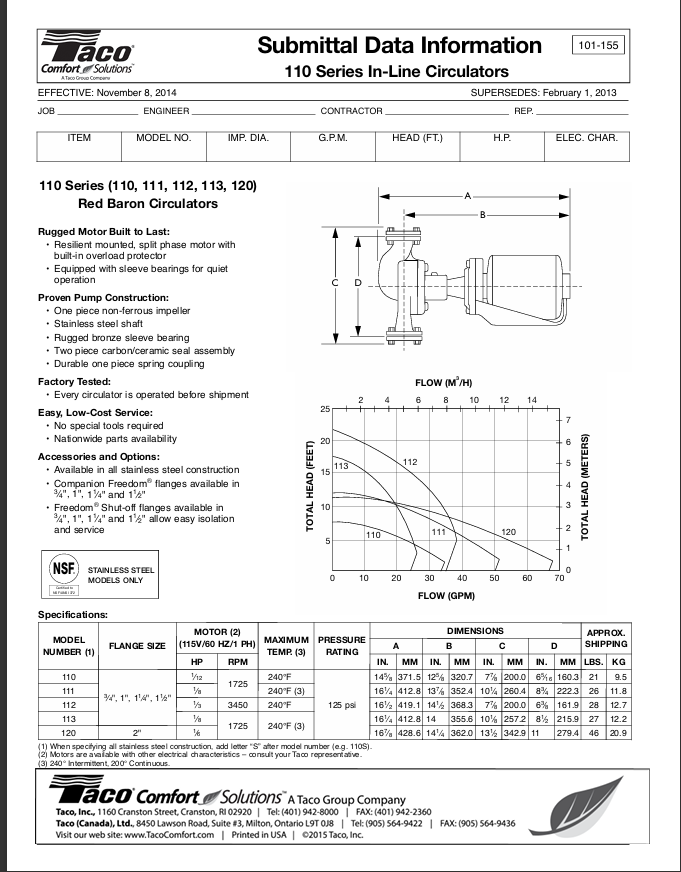
\includegraphics[width=0.9\textwidth]{Questions/Figures/Q2 Pump 2.png}
\end{figure}
\begin{itemize}
    \item Casing size: 1.5'' x 1.5'' x 6 $\frac{5}{16}$ ''
    \item Motor hp: 1/12 hp
    \item Motor speed: 1725 rpm
\end{itemize}

\subsection{Analysis: Maximum Depth}
Maximum depth occures when cavitation will occure for $P_1$ because this is an open loop system.
\begin{align*}
    \text{NPSHA} = \frac{P_s}{\rho g} + \frac{v_{s}^2}{2g} - \frac{P_{\text{vapour}}}{\rho g}
\end{align*}
For pump 1, energy balance assuming $v_1 = v_{s1}$, $z_1 = 0$, $P_1 = P_\text{atm} + \rho g (z_{s_1} - 8)$:
\begin{align*}
    \frac{P_1}{\rho g} + \alpha_1 \frac{v_1^2}{2g} + z_{s_1} & = \frac{P_{s_1}}{\rho g} + \alpha_{s_1} \frac{v_{s_1}^2}{2g} + z_{s_1} + h_{lt, s_1} \\
\end{align*}
Then,
\begin{align*}
    \frac{P_{s_1}}{\rho g} & = \frac{P_\text{atm}}{\rho g} -8 - h_{lt, s_1}
\end{align*}
where
\begin{align*}
    h_{lt} & = h_{1, s_1} + \frac{v^2}{2g} \sum K_L                                                                              \\
           & = \frac{1.5}{100} (z_{s_1} + 220) + \frac{1.8^2}{2 \cdot 32.2} \left(1.25 + 2 \cdot 1.225 + 3 \cdot 0.05 + 1\right) \\
           & = 0.015 z_{s_1} + 3.189
\end{align*}
Then the NPSHA is
\begin{align*}
    \text{NPSHA} & = \frac{P_\text{atm}}{\rho g} - 8 - 0.015 z_{s_1} - 3.189 + \frac{1.8^2}{2 \cdot 32.2} - \frac{P_\text{vapour}}{\rho g} \\ 
    &= \frac{P_\text{atm}}{\rho g} - 8 - 0.015 z_{s_1} - 3.189 + \frac{1.8^2}{2 \cdot 32.2} - \frac{0.3632}{62.3 \cdot 32.2} \cdot \frac{32.2 \; \text{ft}}{1 \; \text{psia}} \cdot \left(\frac{12 \; \text{in}}{1 \; \text{ft}}\right) \\
    &= 21.99 - 0.015 z_{s_1}
\end{align*}
\begin{framed}
Set NPSHA to NPSHR to find the maximum depth:
\begin{align*}
    21.99 - 0.015 z_{s_1} = 10 \implies z_{s_1} = 800 \; \text{ft}
\end{align*}
A depth of 120 ft will not experience cavitation.
\end{framed}

For pump 2, assume $P_3 = P_\text{atm}$, $v_3 = v_{s_2}$, $z_3 = z_{s_2}$. Similarly,
\begin{align*}
\frac{P_{s_2}}{\rho g} &= \frac{P_\text{atm}}{\rho g} - h_{lt, s_2}
\end{align*}
For loss, 
\begin{align*}
    h_{lt, s_2} &= h_{1, s_1} + \frac{v^2}{2g} \sum K_L \\
    &= \frac{1.5}{100} (200) + \frac{1.8^2}{2(32.2)} (0.5 + 2 \cdot 0.05 + 1.225) \\
    &= 3.09
\end{align*}

Then NPSHA is
\begin{align*}
    \text{NPSHA} &= \frac{P_\text{atm}}{\rho g} + \frac{v_{s_2}^2}{2g} - h_{lt, s_2} - \frac{P_{\text{vapour}}}{\rho g} \\
    &= \frac{14.7 - 0.3632}{62.3 (32.2)} \cdot \frac{32.2 \; \text{ft}}{1 \; \text{psia}} \cdot \left(\frac{12 \; \text{in}}{1 \; \text{ft}}\right) + \frac{1.8^2}{2 \cdot 32.2} - 3.09 \\
    &= 33.47 \; \text{ft}
\end{align*}
\begin{framed}
    Pumps of this size don't usually have NPSHR values, so assume NPSHR is 10 ft. Since the NPSHA = 33.47 ft > NPSHR = 10 ft, cavitation will not occur.
\end{framed}
\subsection{Conclusion}
\begin{itemize}
    \item The system is designed with a size of 1.5'' diameter A40 steel pipe.
    \item Large 10hp base-mounted pump. 
    \item Pump suction is lower than 5 fps to avoid erosion.
    \item Pipe may need support anchors between pumps to prevent sagging.
    \item Maximum depth of the pipe inlet is 800 ft before cavitation will occur.
    \item Pumps were oversized to account for changing conditions.
\end{itemize}
\begin{table}[H]
    \centering
    \begin{tabular}{|p{1cm}|p{2cm}|p{2cm}|p{2.5cm}|p{1cm}|p{1cm}|p{1cm}|p{1cm}|p{1cm}|}
        \hline
        Pump & Model & Type & Construction & Flow Rate (gpm) & Fluid & Head Loss (ft) & Motor Size (hp) & Pump Speed (rpm) \\
        \hline
        Pump 1 & Taco, FI/CI, Model 1207D & Centrifugal base mounted & Cast iron 2'' x 1.25'' x 7.25'' & 11 & Water & 140 & 10 & 3500 \\
        Pump 2 & Taco, 110 Series, Model 110 & Centrifugal in-line mounted & Cast iron 1.5'' x 1.5'' x 6 $\frac{5}{16}$ '' & 11 & Water & 5 & 1/12 & 1725 \\
        \hline
    \end{tabular}
\end{table}